
\chapter{Example}
\label{cha:example}

We want to examine a specific problem to demonstrate differences in Dynamic Programming and Reinforcement Learning. The parking problem \cite{bertsekas2019reinforcement} can be seen as a fully defined finite Markov Decision Process and therefore has an optimal analytical solution but also fits well to be solved by policy approximation methods such as Q-Learning \ref{subsec:ql}.

\section{Parking Problem}
\label{sec:parking_problem}

This problem describes a series of sequentially placed parking spaces. The driver starts at place $0$ and traverses the spaces sequentially until parking at a space or reaching the last space $N$ and parking in the garage. The driver can only observe the current parking place, free with an independent probability $p(i)$. The driver can park in a free place using the cost function $c(i)$ describing the distance the driver has to walk to his destination. Parking in the garage has a fixed cost $C$ and no walking cost. We want the optimal policy to minimize the expected costs for a driver.\\

\begin{figure}[htp]
	\centering
	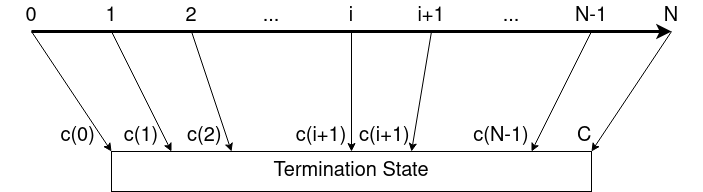
\includegraphics[scale=0.55]{figures/parking_graphic.png}
	\caption{State transitions and costs of the Parking Problem}
\end{figure}

\begin{itemize}
	\item $N$: Number of parking spaces
	\item $p(i)$: Probability that parking space $i$ is free
	\item $c(i)$: Cost of the parking space $i$
	\item $C$: Cost of the garage
\end{itemize}
This problem gives us a total of $2N+1$ states as for each parking place, we need one state for the place being free and one for being taken. We also need an end state indicating that the driver has parked. 

This problem is stochastic as it is uncertain what the next state will be after a transition. For simplicity, we will assume a constant $p$, but the following solutions can also be expanded to handle a function $p(i)$.

\section{Practical Example}
\label{sec:practical}
We will now look at concrete values to compare different approaches to solving the stochastic Markov Decision Process with the following parameters.

The probability of a parking space being free will be constant. The cost function will increase linearly with the space index. We will set the garage cost to half of the number of spaces.
\begin{itemize}
	\item $p(i) = p$
	\item $c(i) = N-i$
	\item $C = \frac{N}{2}$
\end{itemize}

As the cost function is linear and $c(0) > C > c(N)$, we can already expect that the best policy will be to drive up until a certain point and then park at the next free space. Therefore the policy will take the action drive for all states before this threshold and then changes to park at reaching the threshold space.

\begin{figure}[htp]
	\label{figure}
	\centering
	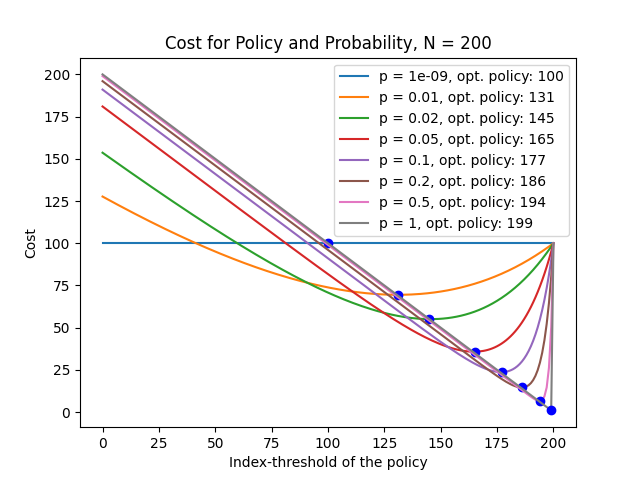
\includegraphics[scale=0.6]{figures/code_statistics/strategy_probabilities_200.png}
	\caption{Cost of per policy and probability for the parking problem}
\end{figure}
We can note from this figure \ref{figure} that the optimal policies and, therefore, costs are linearly dependent on the constant probability of a parking space being free. The expected result if all places are free is to park at the last possible index. If nearly every place is taken, the best policy is to try parking at space $\frac{N}{2}$ as this is at most as bad as parking in the garage.


\subsection{Dynamic Programming Approach}
\label{subsec:dp_approach}
As the entirety of the model is given, we can easily set up an analytical solution using Bells equation \ref{eqn:sto_bellman}. It is crucial to notice that the value of a state does not depend on whether the previous place was free or taken. It depends only on the current index and already considers that this place is possibly taken.

The maximum from the 2 possible actions can be simplified as one already translates to the terminal state ending the recursion. We use $\gamma = 1$ as this gives the optimal solution regarding fully weighted future costs. 

\subsubsection{Recursive Value Function}
\begin{equation*}
	\begin{split}
		&V(N) = C = \frac{N}{2}\\
		&V(i) = p(i) \cdot c(i) + (1-p(i)) \cdot V(i+1)\\
		&0 \leq i < N 
	\end{split}
\end{equation*}

\subsubsection{Explicit Value Function}
\begin{equation}
	\begin{split}
		&V(i) = C \cdot (1-p)^{N-i} + \sum_{j=0}^{N-i} p \cdot (N-i-j) \cdot (1-p)^{j}
	\end{split}
\end{equation}


Now that we have calculated the optimal cost using the entire model, we will approximate this solution using Q-Learning, a model-free algorithm.

\subsection{Q-Learning Approach}
\label{subsec:ql_approach}
Q-Learning does not need to know any probabilities or state transitions. However, it will learn to take actions that will approximate the optimal cost arbitrarily close given enough training steps. 

Therefore the remaining model parameters we need to know are all states, possible actions, and the reward from transitions.

\subsubsection{Reward Function}
Q-Learning tries to maximize the reward in contrast to Dynamic Programming, which minimizes the cost. Therefore we need to transform our cost function into a corresponding reward function. 
We negate the cost function and garage cost \ref{sec:practical} and, as Q-Learning needs positive numbers, level the reward function and garage reward to be all positive by adding $N$.

\begin{itemize}
	\item $C \rightarrow R = \frac{N}{2}$
	\item $c(i) \rightarrow r(i) = i$
\end{itemize}

This function only rewards taking the action to park. We can instead reward transitions and give iterative rewards. It needs to hold that the sum of rewards received upon parking in any space stays equal. However, rewarding actions directly improves the performance of the Q-learning algorithm. An equally performative policy can be trained with fewer iterations than by rewarding the parking action. The following incremental reward function reduces the necessary iterations in learning to less than half of the aggregated reward function above.

\begin{itemize}
	\item Reward from driving forward: $r(i+1) - r(i) = 1$
	\item Reward from transitioning to the garage: $-\frac{N}{2}$
\end{itemize}

\subsubsection{Parameters}
These parameters work well with both reward functions
\begin{itemize}
	\item $\alpha_0 = 0.05$
	\item $\gamma = 0.999$
	\item $\epsilon_0 = 0.05$ 
\end{itemize}
To improve convergence speed, we use a descending learning rate $\alpha_i$ and exploration rate $\epsilon_i$. With $i$ being the current iteration and $n$ being the number of overall iterations.
\begin{itemize}
	\item $\alpha_i = \alpha_0 \frac{n - i + 1}{n}$
	\item $\epsilon_i = \epsilon_0 \frac{n - i + 1}{n}$
\end{itemize}
\subsubsection{Learning Progress}
For space sizes larger than $500$ the learning rate can be increased while keeping the learning stable. Depending on the space size, the number of iterations also needs to be increased.
For $N=200$ and $p = 0.05$ it is enough to have $60000$ learning iterations for stable results.

Using incremental rewards and diminishing learning and exploration rate, the algorithm converges at about $40000$ training iterations. The plotted cost estimates are averaged from $20000$ samples using the current Q-Table policy.

\begin{figure}[htp]
	\centering
	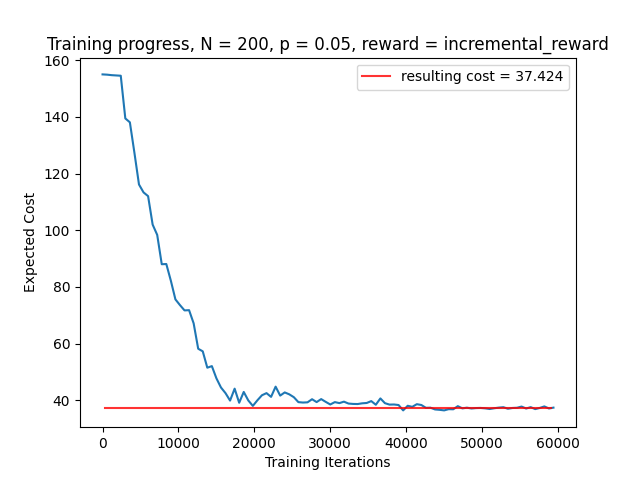
\includegraphics[scale=0.6]{figures/code_statistics/q_training_progress_200.png}
	\caption{Training Progress of Q-Learning Problem, $\alpha_0 = 0.05$, $\epsilon_0 = 0.05$, $\gamma = 0.999$}
\end{figure}

\FloatBarrier

\subsubsection{Results}
Q-Learning can approximate the Dynamic Programming solution quite well. The solution could be better approximated by using a better reward function, tuning the parameters, and increasing the training cycles.
These results use the incremental reward function, a linearly descending learning and exploration rate.

\begin{center}
	\begin{tabular}{ |c|c|c|c| } 
		\hline
		N& \multicolumn{2}{c|}{Q-learning} & Dynamic Programming\\ 
		\hline
		-& mean & standard deviation & -\\ 
		\hline
		$50$ & $17.005$ & $0.263$ & $16.366$ \\ 
		\hline
		$100$ & $26.251$ & $0.519$ & $25.140$ \\ 
		\hline
		$200$ & $37.145$ & $0.989$ & $35.764$ \\ 
		\hline
		$500$ & $53.973$ & $1.591$ & $51.663$ \\ 
		\hline	
	\end{tabular}\\
\end{center}

The results for Q-learning are calculated from 20 learning results, each parking space randomly free with a probability of $0.05$.
